\section{Comparing PageRank, HITS and SALSA} \label{sec:compare}
\subsection{Spamdexing}
Spamdexing is an intentional attempt to improve the ranking of a page on a SE, this can be done by link spam or by link farms, as shown in Figure \ref{fig:link farm}. 
\begin{figure}[h!]
\centering
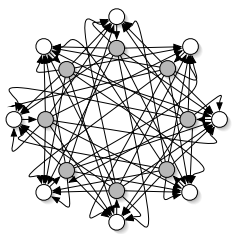
\includegraphics[width=5cm]{link_farm_baldi.png}
\caption{A link farm, where the shaded nodes are all copied of the same page, taken from \cite{baldi2003modeling}}
\label{fig:link farm}
\end{figure}

PR is sensitive to in-degree and so a simple way to spamdex PR is to increase the in-degree to your page. \cite{bonato} As HITS and SALSA are less sensitive to spamdexing than PR. 

\subsection{Dual Rankings}
An advantage of HITS compared to PR is the dual ranking that is assigned to each web page, a user might find this useful to find out which pages are the most authoritative on a query topic.

SALSA also has dual rankings as does HITS, and is also query dependant, making it computationally less taxing than PR \cite{langville}.


\subsection{Query-dependence}
HITS is also query-dependant, it first generates a root set dependant on the query, and returns two real numbers for a given page HITS deems relevant to the topic, however PR returns a rank for each page in the whole web graph, this is also a weakness of the algorithm, as the computation required to produce the dual rankings must occur at query time. It is possible to make HITS query dependant by removing the sampling step of the algorithm, hence reducing computation time. 

\subsection{Uniqueness}
A problem can arise with the uniqueness of the vectors produced, as different authority and hub vectors are computed by different choices of the initial vector \cite{langville}. Output of HITS depends on weather the implementation uses the initial authority or hub vector \cite{farahat2006authority}. HITS converges to a non-unique solution as the authority matrix is not irreducible, we are able to modify HITS in a manner similar to the primitivity adjustment in PR, as discussed in section \ref{sec:matrix}. In this modification, we can create a modified authority matrix \(\xi\textbf{L}^T\textbf{L} +\frac{(1-\xi)}{n}\textbf{ee}^T\) can be created, where $0<\xi<1$ \cite{ng2001stable}, and similarly create a hub matrix, \(\xi\textbf{LL}^T +\frac{(1-\xi)}{n}\textbf{ee}^T\) . These modified matrices are now irreducible, and by the Perron-Frobenius theorem, we can find a unique, normalised, positive dominant eigenvector \cite{meyer2000matrix}. This adjustment also solves the problem arising with pages having the same rank, for example in Table \ref{Table:HITS}, nodes 2 and 6 both have the same rank in terms of their authority.

SALSA can give inconsistent hub and authority rankings due to non-uniqueness \cite{farahat2006authority}.

HITS and SALSA eigenvectors do not have to be unique, whereas for PR they do. HITS and SALSA can now behave unexpectedly, as the output depends on the initial seed vector, PR doesn't display this inconsistency \cite{farahat2006authority}. A ranking algorithm that assigns both hub and authority weights is badly behaved on G if the final results is dependant on on initial vectors, or if a node is given authority or hub weight of zero, even if it has either an in-degree or out-degree which is greater than zero \cite{bonato}. %This occurs in our example at nodes 2h and 6h, they are given an in-link weight of zero, as the only in-link is from node 1a, which also has a weight of 0.  

\subsection{Topic Drift}

Topic drift has been shown to be avoided by using topic vectors to filter N, a topic vector is a term vector which has been computed from the text of pages in the base set, a page is only able to remain in N if its term vector is a good match to this topic vector. \textcolor{red}{\textbf{EXPLAIN MORE HERE}}

SALSA, is less impacted by topic drift \cite{lempel2000stochastic}, and is less susceptible to spamming, the coupling between the hub and authority scores is less strict in SALSA. However HITS and SALSA are easier to spam than PR due to the mutual reinforcement effect \cite{langville}. 

\subsection{Computation costs}
A weakness of PR is that the web contains many documents that calculations must be done on many computers, also the structure and content of the web changes daily, leading to the 'Google Dance' which must be done monthly \cite{thorson2004modeling}. 

HITS is usually described as running on a smaller collection of articles that have been retrieved on a query topic, whilst PR runs on the entire web \cite{ng2001link}. As we form \textbf{L} through the base set, the order of \textbf{L} is much smaller then the total number of pages on the web, and so the computation required in producing a ranked list of the web pages is less costly than the computation in PR, we also do not need to compute eigenvectors for both matrices, as we are able to use the equations, which is also computationally simpler. 

Figure \ref{fig:N build} shows how the N graph that is built through the HITS algorithm is smaller than the web graph, and so it is less computationally taxing on a system.

\begin{figure}[h] 
\centering
\begin{tikzpicture}[->,>=stealth',shorten >=1pt,auto,node distance=2cm,
semithick]
\tikzstyle{every state}=[fill=white,draw=black,text=black]
\node[state] (1) {$1$};
\node[state] (2) [right of=1] {$2$};
\node[state] (3) [right of=2] {$3$};
\node[state] (4) [below of=2] {$4$};
\node[state] (5) [below of=3] {$5$};
\node[state] (6) [below of=4] {$6$};
\path (1) edge node{} (2)
          edge [bend left] node{} (3)
          edge node{} (4)
          edge node{} (6)
      (2) edge node{} (4)
      (3) edge node{} (2)
          edge node{} (4)
          edge node{} (5)
      (4) edge node{} (5)
      (6) edge node{} (5)
          edge node{} (4);
\end{tikzpicture} \qquad\qquad
\begin{tikzpicture}[->,>=stealth',shorten >=1pt,auto,node distance=2cm,
semithick]
\tikzstyle{every state}=[fill=white,draw=black,text=black]
\node[state] (1) {$1$};
\node[state] (2) [ultra thick, right of=1] {$2$};
\node[state] (3) [right of=2] {$3$};
\node[state] (4) [below of=2] {$4$};
\node[state] (5) [ultra thick, below of=3] {$5$};
\node[state] (6) [below of=4] {$6$};
\path (1) edge node{} (2)
      (2) edge node{} (4)
      (3) edge node{} (2)
          edge node{} (5)
      (4) edge node{} (5)
      (6) edge node{} (5);
\end{tikzpicture}
\caption{Neighbourhood graph, N,  for {2,5}} \label{fig:N build}
\end{figure}


\subsection{TKC Effect}
There are three main problems which can arise through using connectivity analysis on web pages, such as mutually reinforced relationships in a tightly knitted community, TKC, where a set of documents on page A could point to a single document on page B which would then drive up the hub score of page A, whilst increasing the authority ranking on page B, when this occurs in the TKC, pages that may have no authority on a topic or may pertain to just one aspect of the query may score high undeservedly \cite{lempel2000stochastic}. There is also a problem of automatically generated links, which would not represent human opinion, also topic-drift arises through the usage of connectivity analysis, where when building N, it is possible for an authoritative page which is off-topic can be linked to pages which contain the query term, and so can skew the rankings to off-topic pages. The general solution to this problem as suggested by Bharat and Herzinger is to use content analysis \cite{bharat1998improved}. Using this improved algorithm, precision over the original HITS algorithm has been shown to increase by 45\%, however this is limited to topics that are already well-represented and connected on the web. 

'It is this combination of a site’s intra-community authority score and its community’s size that allows the stochastic approach to blend authorities from different aspects of a multi-topic query, and which reduces its vulnerability to the TKC effect.We have shown that the ranking produced by SALSA is equivalent to a weighted in=out-degree ranking (with the sizes of irreducible components also playing a part). This makes SALSA computationally lighter than the mutual reinforcement approach. We note that SALSA is less vulnerable to the TKC effect, and produces good results in many cases where the mutual reinforcement approach fails to do so.\cite{lempel2000stochastic}'

HITS emphasises the mutual reinforcement between authority and hub web pages, whereas PR focuses more on web surfing based on random walk models HITS emphasises the mutual reinforcement between authority and hub web pages \cite{ding2003pagerank}.

\subsection{Sensitivity}

HITS is insensitive to minor changes in its neighbourhood graph, N, PR can be sensitive depending on where the change occurred. If the change in the web graph occurred with pages that have a low PR value, then the overall PR is very small \cite{bonato}.

\begin{table}[H] \caption{Page rankings for Figure \ref{fig:Example} using PR, HITS and SALSA }
 \centering
 \begin{tabular} {c| c| c| c| c| c} 
 \multirow{2}{*}{Node} & \multirow{2}{*}{PR} & \multicolumn{2}{|c|}{HITS} & \multicolumn{2}{|c}{SALSA} \\ [0.5ex] 
 {}&{}&Authority & Hub & Authority & Hub\\ 
 \hline
 1&8&8&6&3&1\\
 2&6&6&4&6&3\\
 3&5&5&5&6&7\\
 4&4&3&1&3&3\\
 5&2&1&7&1&7\\
 6&6&6&3&6&1\\
 7&3&2&8&2&3\\
 8&1&4&1&2&3\\
 \end{tabular}
 \label{Table: comparison}
\end{table}
